\documentclass{homeworg}
\usepackage{mathtools}
\usepackage{tikz}
\usepackage{biblatex}
\addbibresource{mybibliography.bib}
\title{CS31920 Advanced Algorithms Assignment: Applying Linear Programming }
\author{Oisín Brady [oib]}

\begin{document}

\maketitle

\section{Introduction}
The problem involves a rectangular puzzle grid. Each field of the grid contains either a color or is empty. For all fields with a color there is exactly one other field that contains the same color, such that each color appears exactly twice in the grid. It is required to draw a path connecting each color pair simultaneously such that: each step in the path is a non-diagonal step towards an adjacent field, each field contains \textit{at most} one mark denoting it is part of a connection (i.e. for each field of a colored path, p, none of the fields of another colored path are in common with p). The following figures are extracts from the assignment brief [CITATION NEEDED?]:

\hspace*{-2.5em}
\begin{figure}[h]
        \centering
        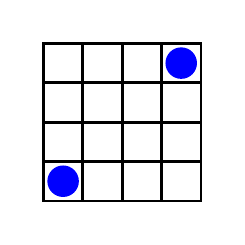
\begin{tikzpicture}[line width=1pt]
                \path  (-0.2, -0.2) rectangle (2.2, 2.2);
                \draw (0, 0) rectangle (2, 2);
                \foreach \i in {0.5, 1.0, ..., 1.5} {
                        \draw (0, \i) -- (2, \i);
                        \draw (\i, 0) -- (\i, 2);
                }
                \fill[blue] (0.25, 0.25) circle (0.2);
                \fill[blue] (1.75, 1.75) circle (0.2);
        \end{tikzpicture}
        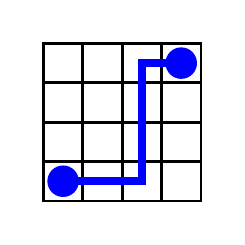
\begin{tikzpicture}[line width=1pt]
                \path  (-0.2, -0.2) rectangle (2.2, 2.2);
                \draw (0, 0) rectangle (2, 2);
                \foreach \i in {0.5, 1.0, ..., 1.5} {
                        \draw (0, \i) -- (2, \i);
                        \draw (\i, 0) -- (\i, 2);
                }
                \fill[blue] (0.25, 0.25) circle (0.2);
                \fill[blue] (1.75, 1.75) circle (0.2);
                \draw[blue, line width=3pt] (0.25, 0.25) -- (1.25, 0.25) -- (1.25, 1.75) -- (1.75, 1.75);
        \end{tikzpicture}
        \\
        \caption{left: puzzle input, right: valid solution.}
\end{figure}

\begin{figure}[h]
    \centering
    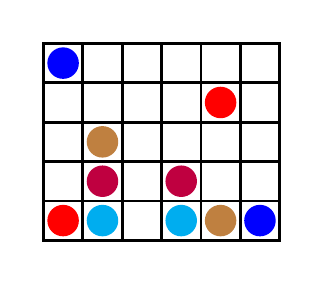
\begin{tikzpicture}[line width=1pt]
            \path  (-0.2, -0.2) rectangle (3.2, 2.7);
            \draw (0, 0) rectangle (3, 2.5);
            \foreach \i in {0.5, 1.0, ..., 2} {
                    \draw (0, \i) -- (3, \i);
                    \draw (\i, 0) -- (\i, 2.5);
            }
            \draw (2.5, 0) -- (2.5, 2.5);
            \fill[blue] (0.25, 2.25) circle (0.2);
            \fill[blue] (2.75, 0.25) circle (0.2);
            \fill[red] (0.25, 0.25) circle (0.2);
            \fill[red] (2.25, 1.75) circle (0.2);
            \fill[brown] (0.75, 1.25) circle (0.2);
            \fill[brown] (2.25, 0.25) circle (0.2);
            \fill[cyan] (0.75, 0.25) circle (0.2);
            \fill[cyan] (1.75, 0.25) circle (0.2);
            \fill[purple] (0.75, 0.75) circle (0.2);
            \fill[purple] (1.75, 0.75) circle (0.2);
    \end{tikzpicture}
    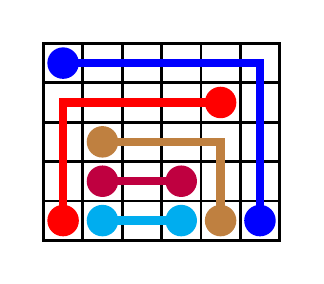
\begin{tikzpicture}[line width=1pt]
            \path  (-0.2, -0.2) rectangle (3.2, 2.7);
            \draw (0, 0) rectangle (3, 2.5);
            \foreach \i in {0.5, 1.0, ..., 2} {
                    \draw (0, \i) -- (3, \i);
                    \draw (\i, 0) -- (\i, 2.5);
            }
            \draw (2.5, 0) -- (2.5, 2.5);
            \fill[blue] (0.25, 2.25) circle (0.2);
            \fill[blue] (2.75, 0.25) circle (0.2);
            \draw[blue, line width=3pt] (0.25, 2.25) -- (2.75, 2.25) -- (2.75, 0.25);
            \fill[red] (0.25, 0.25) circle (0.2);
            \fill[red] (2.25, 1.75) circle (0.2);
            \draw[red, line width=3pt] (0.25, 0.25) -- (0.25, 1.75) -- (2.25, 1.75);
            \fill[brown] (0.75, 1.25) circle (0.2);
            \fill[brown] (2.25, 0.25) circle (0.2);
            \draw[brown, line width=3pt] (0.75, 1.25) -- (2.25, 1.25) -- (2.25, 0.25);
            \fill[cyan] (0.75, 0.25) circle (0.2);
            \fill[cyan] (1.75, 0.25) circle (0.2);
            \draw[cyan, line width=3pt] (0.75, 0.25) -- (1.75, 0.25);
            \fill[purple] (0.75, 0.75) circle (0.2);
            \fill[purple] (1.75, 0.75) circle (0.2);
            \draw[purple, line width=3pt] (0.75, 0.75) -- (1.75, 0.75);
    \end{tikzpicture}
    \\
    \caption{left: puzzle input, right: valid solution.}
\end{figure}

The remainder of this report will discuss the following; the translations necessary to model the puzzle into a maximum flow problem; designing a linear program to solve the maximum flow problem; the implementation of the model written in the C programming language; a conclusion which reflects on the approach used to solve this problem and whether I am happy with its outcome.

\newpage
\section{Modelling}
The problem can be modelled as a maximum flow problem before being solved via linear programming.
Reducing to a maximum flow problem requires translating the introduced problem into the key components of a maximum flow problem. Namely: a flow network, a flow, a value of flow, and an objective. 
\subsection{Translating Problem to a Flow Network}
The definition of a maximum flow problem is split into two sections, its input and output. The following will present these definitions before showing how the puzzle problem is translated into the input of a maximum flow problem, and how the output is produced via linear programming.
\subsubsection{Input Definition}
An asymmetric, weighted, directed graph \(G = (V, E, c)\) with source node \(s \in V\), sink node \(t \in V\), and positive edge capacities \(c:E\rightarrow R+\). A source has no incoming edges \((v,s) \notin E \text{ for all } v \in V\). Asymmetric means \((v,w) \in E \implies (w,v) \notin E\). [DO I NEED SLIDE CITATION?]
\subsubsection{Translating Problem to Max Flow Input}
Let each field in the puzzle grid be a node in graph G. Based of the input grid, nodes are identified by a positive non-zero integer no greater than n, where n is the total number of fields in the input puzzle. The ordering of the node identifiers start with 1 at the top left node and ends at the bottom right node n, with the sequence progressing as if reading from a book.\\

\begin{figure}[h]
        \centering
        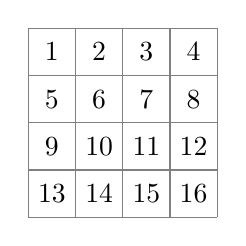
\begin{tikzpicture}[scale=1.2]
            \draw[step=0.5cm,color=gray] (-1,-1) grid (1,1);
            \node at (-0.75,+0.75) {1};
            \node at (-0.25,+0.75) {2};
            \node at (+0.25,+0.75) {3};
            \node at (+0.75,+0.75) {4};
            \node at (-0.75,+0.25) {5};
            \node at (-0.25,+0.25) {6};
            \node at (+0.25,+0.25) {7};
            \node at (+0.75,+0.25) {8};
            \node at (-0.75,-0.25) {9};
            \node at (-0.25,-0.25) {10};
            \node at (+0.25,-0.25) {11};
            \node at (+0.75,-0.25) {12};
            \node at (-0.75,-0.75) {13};
            \node at (-0.25,-0.75) {14};
            \node at (+0.25,-0.75) {15};
            \node at (+0.75,-0.75) {16};
            
        \end{tikzpicture}
        \\
        \caption{Identifiers for each node in a 4x4 input puzzle grid}
\end{figure}

For each pair of nodes of the same color (matching dots in figures 1 \& 2), one is arbitrarily selected as the source node and the other as the sink node. An edge is introduced for each color for each connection between non-diagonally adjacent fields (nodes) in the puzzle grid. For example, if a puzzle has two color pairs represented by the integers 1 and 2, then for every edge not involving a source or sink node, we would introduce the same edge for each color. The edge between (non-source/sink) adjacent nodes 3 and 4 in figure 3 would produce the following edges: e(3,4,1), e(3,4,2), where the first two values of edge, e, represent the nodes connected by an edge and the last value represents the color. Edges are not introduced if they would be incoming edges to a source node. Similarly, with sink nodes, edges are not introduced if they would be outbound edges from a sink node.\par
\newpage
It is unclear what direction a path to a valid solution will be. Also, it is feasible that  multiple variations of one or more paths exist in a puzzle. Therefore, we must first produce a symmetric graph in our input, otherwise we would be limiting the solution space to our problem (potentially deeming a feasible solution infeasible). This violates the asymmetric requirement of our maximum flow input. However, we can restrict drawing a connection between nodes in paths if the connection goes into a node that is already part of a path. This restriction can be emplaced by the linear program described later in sections 2.1.4 and 2.1.6. \par
The positive edge capacities are introduced as bounds of the linear program that will later be described in sections 2.1.4 and 2.1.6.\par


\subsubsection{Output Definition}
\begin{enumerate}
    \item[(1)] A flow \(f:E\rightarrow \mathbb{R}_0^+\) that respects the capacity constraints:
        \begin{enumerate}
        	\item[] \(f(e)\leq c(e) \text{ for all } e \in E\)
        \end{enumerate}
    \item[(2)] Guarantees flow conservation at all nodes except source and sink: 
        \begin{enumerate}
        	\item[] \(\displaystyle\sum_{u \in V} f(u, v) = \sum_{w \in V} f(v, w) \text{ for all }v\in V \text{\textbackslash} \{s, t\}\)
        	\end{enumerate}
	\item[(3)] Maximises the value:
        \begin{enumerate}
        	\item[] \(v(f)=\displaystyle\sum_{v \in V}f(s, v)\)
        \end{enumerate}
\end{enumerate}
\subsubsection{Translating Problem to Max Flow Output (Using LP)}
A linear program outputs a solution to the puzzle, if possible. The LP respects the capacity constraints, flow conservation, along with additional constraints specific to this problem (highlighted below). The linear program's goal is to maximise the total flow leaving the source node(s).\par
\(\text{Maximise} \displaystyle\sum_{v \in V, (s,v) \in E}x_e \text{ for all source nodes, s}\\
S.t\\\)
\begin{enumerate}
    \item[(1)] 
        \begin{enumerate}
        	\item[] \(x_e \leq 1 \text{ for all }e \in E\)
        \end{enumerate}
    \item[(2)]
        \begin{enumerate}
        	\item[] \(\displaystyle\sum_{u \in V}x_(u,v) = \displaystyle\sum_{w \in V}x_(v,w) \text{ for all } v \in V \text{\textbackslash} \{s, t\} \)\
        \end{enumerate}
    \item[(3)] 
        \begin{enumerate}
        	\item[] \(\displaystyle\sum_{u \in V}x_(u,v) \leq 1 \text{ for all } v \in V \text{\textbackslash} \{s\} \)\
        \end{enumerate}
    \item[(4)] 
        \begin{enumerate}
        	\item[] \(\displaystyle\sum_{u \in V}x_(u,v) = \displaystyle\sum_{w \in V}x_(v,w) \text{ for all } v \in V \text{\textbackslash} \{s, t\}, \text{where, } x(u,v)_{color} = x(u,w)_{color} \)\
        \end{enumerate}
    \item[(5)] 
        \begin{enumerate}
        	\item[] \(x_e \geq 0 \text{ for all } e \in E\)
    \end{enumerate}
\end{enumerate}

Where,
\begin{enumerate}
    \item[] \(X_e\) denotes the flow value of each edge in the graph, introduced in section 2.1.2.
    \item[] \(v_{color}\) denotes the what source-sink pair this edge is part of (described earlier in section 2.1.2)
\end{enumerate}

\subsubsection{Objective function}
The objective function calls to maximise the sum of the flow values leaving all source nodes. Since all edges have a capacity <= 1 (1), and all paths are non-branching (3), a valid solution is one in which the objective value = the number of color pairs in the input puzzle grid. This is equivalent to saying that a valid solution is one in which all paths between color pairs can be drawn simultaneously.

\subsubsection{Constraints}
\begin{enumerate}
    \item[(1)] Ensures that the flow value of each edge respects the capacity by not exceeding a flow value of 1. This constraint, combined with (5) constructs the bound for all edges, e, so that e = [0,1]. This means that edges will either be part of a color pair path or not (the program will later dismiss fractional values).
    \item[(2)] Ensures the law of flow conservation. This means that the total incoming flow of a node must be equivalent to its total outgoing flow. This does not apply for the source or sink node as sinks only have incoming edges and sources only have outgoing edges
    \item[(3)] Ensures that paths do not branch. I.e., by ensuring that all edge flow values are at most 1, we avoid having paths that split into separate paths or multiple paths merging into one (The implementation will disregard fractions, effectively making the edge flow value all or nothing (either 1 or 0)).
    \item[(4)] Ensures that the paths between different colors do not share nodes.
    \item[(5)] Ensures that edge values are at least 0. Used in combination with (1) to produce a bound for all edges.
\end{enumerate}

\section{Implementation}
The implementation is written in C and the linear program is constructed and solved using the GLPK library\cite{1}. My section of the program (that which was not already featured in the template code provided in the "puzzleSolver.c" file) involves the following process:\\
\begin{enumerate}
    \item[1:] Creating an LP problem object with the objective function set to maximisation
    \item[2:] Creating an adjacency matrix based of the input file (already handled in puzzleSolver.c template code) that maps all possible edges between nodes in the puzzle grid. The adjacency matrix is later used to determine what edge variables are introduced which in turn are used in the linear program. All of these edges are given constraints depending on their involved nodes and the color pair they belong to.
    \item[3:] Creating all LP bounds (combined (1) \& (2) of section 2.1.4, implemented using glpk functions)
    \item[4:] Creating all LP constraints (See section 2.1.4) for each node (using glpk functions).
    [MORE DETAIL - perhaps some example code lines] 
    \item[5:] Solving glpk LP via the Simplex algorithm (using a glpk function).
    \item[6:] Determining whether a "solved" optimal solution draws all paths between color pairs simultaneously. I.e., determine if the input puzzle is solvable or not.
\end{enumerate}


\section{Discussion and Conclusion}

Alternatively, by the notion of local replacement [CITE WEEK 4 LECTURE 1 SLIDE 182], an additional node could be introduced for each non-source/sink node to allow for paths between itself and its adjacent nodes in both directions. [ADD THIS SENTENCE TO DISCUSSION \& CONCLUSION SECTION]

\section{References}

\printbibliography


\end{document}
